\documentclass[11pt,french]{article} % police taille 11 car 10 c'est pour les terroristes
\usepackage{babel} % paquet qui permet de gérer les différentes langues
\usepackage{graphicx} % paquet pour inclure des images
\usepackage{float}
\usepackage{titling}
\usepackage{environ}
\usepackage{amsmath,amsfonts,amssymb,amsthm}
\usepackage{geometry}
\geometry{legalpaper, margin=100pt}

\setlength{\parindent}{0pt}

\NewEnviron{NORMAL}{% environnement used to scale math equations 
    \scalebox{1.2}{$\BODY$} 
} 

\begin{document}

\begin{figure}[t]
    \centering
		\advance\leftskip-0.2cm
    
\includegraphics[width=8cm]{inp_n7.png} % joli logo de l'N7
\end{figure}

\title{\vspace{0.5cm} \textbf{Rapport de bureau d'études\\Automatique Systèmes Cyber Physique}} 
\author{RAGOT Cyrian}
\renewcommand{\maketitlehookc}{%
	\vspace{3cm}
  \begin{center}
		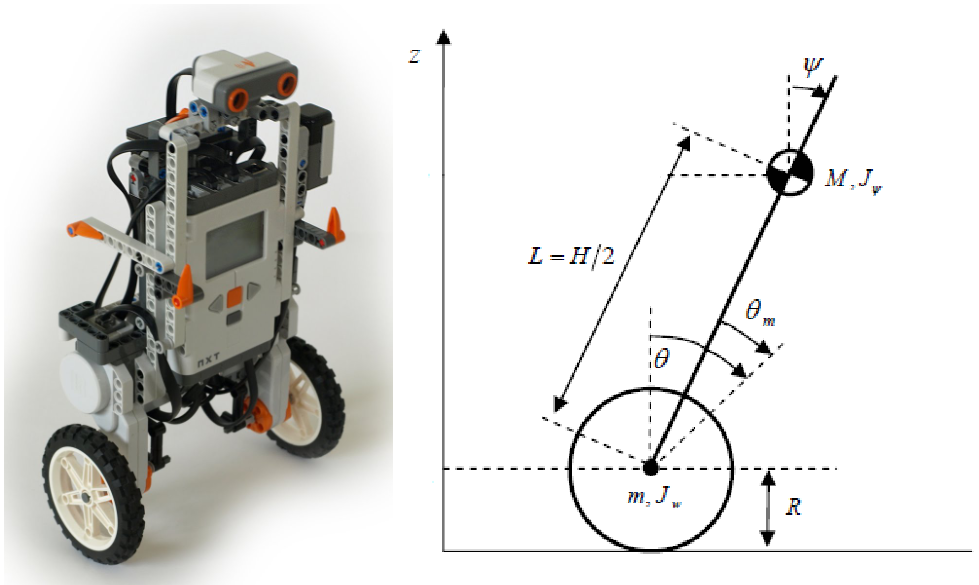
\includegraphics[width=14cm]{segway.png} % image segway 1ere page
  \end{center}
}
\date{\vspace{1cm}\vfill Département Sciences du Numérique - Première année \\
2023-2024 }

\maketitle

\newpage % génère un saut de page, en gros retour à la ligne mais pour une page
\tableofcontents % génère un sommaire des sections du document
\newpage

\section{Introduction}


\newpage
\section{Modèle du pendule inversé}
\subsection{Contrôle par retour d'état}

Dans cette partie, nous étudierons un modèle simple d'un pendule inversé contrôlé par retour d'état (figure \ref{fig:schema_pend_inv}) pour lequel on a accès aux variables de sortie. Le système contrôlé issu des équations physiques de la dynamique est \\


\begin{equation}
	\NORMAL{
  \left\{
    \begin{array}{l}
			\dot{x}_1(t) = x_2(t) \\
			\dot{x}_2(t) = \frac{g}{l}sin(x_1(t))-\frac{cos(x_1(t))u(t)}{l} \\
			\dot{x}_1(0) = x_{0,1} = \alpha_0 \\
			\dot{x}_2(0) = x_{0,2} = \dot\alpha_0, \\
    \end{array}
  \right.
	}
\end{equation}\\

avec

\begin{description}
	\item[--] $\mathbf{g = 9.81 m/s^2}$ constante de gravité
	\item[--] $\mathbf{l = 10 m}$ longueur du pendule
	\item[--] $\mathbf{t_0 = 0 s}$ instant initial
	\item[--] $\boldsymbol{x(t) = (x_1(t), x_2(t))^\intercal = (\alpha(t), \dot\alpha(t))^\intercal}$ variable d'état 
	\item[--] $\boldsymbol{(x_e,u_e)^\intercal = (0,0,0)^\intercal}$ point de fonctionnement
	\item[--] $\boldsymbol{u(t)}$ contrôle par retour d'état
\end{description}

\begin{figure}[h]
    \centering
		\advance\leftskip-0.2cm
    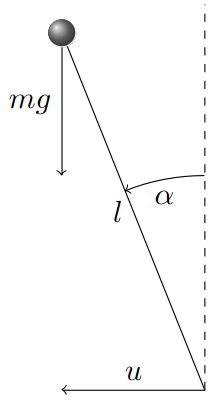
\includegraphics[width=3cm]{pendule_inverse.png} % joli logo de l'N7
		\label{fig:schema_pend_inv}
		\caption{Schéma du pendule inversé}
\end{figure}
\vspace{0.5cm}

\subsubsection{Analyse du modèle théorique}

L'équation d'état est alors

\begin{equation}
	\NORMAL{
			\dot{x}(t) = f(x(t),u(t)), \\
	}
\end{equation}\\

où 

\begin{equation}
	\NORMAL{
		f(x,u) = 
		\left(
		\begin{array}{c}
			x_2 \\
			\frac{g}{l}sin(x_1)-\frac{cos(x_1)u}{l} \\
    \end{array}
  \right)
	}
\end{equation}\\


On souhaite stabiliser le système à l'origine (la position verticale du pendule inversé), cependant le système non contrôlé n'est pas stable à l'origine. En effet, lorsque $u = 0$, en passant par la jacobienne de $g$ au point de fonctionnement puis son polynôme caractéristique, on trouve la valeur propre $\sqrt{\frac{g}{l}}$ qui est à partie réelle strictement positive.\\

% TODO : on pourrait parler du critere de Kalman si ya de la place encore
% TODO : on pourrait mettre des equations pour le calcul de la vp aussi

On choisit alors un contrôle en boucle fermée par retour d'état linéaire de la forme $u(t) = u_e + K(x(t) - x_e)$ avec $K = (k_1, k_2)$. Cherchons alors $K$ de manière à avoir un contrôle qui stabilise le système asymptotiquement en $x_e$.\\

On boucle le système :\\

\begin{equation}
	\NORMAL{
			\dot{x}(t) = f(x(t),u_e + K(x(t)-x_e)) := g(x(t)) \\
	}
\end{equation}\\

Alors $g(x_e) = f(x_e, u_e) = 0$ donc $x_e$ est un point d'équilibre de $\dot{x} = g(x)$. \\

La matrice jacobienne associée est alors 

\begin{equation}
	\NORMAL{
		J_g(x) = 
		\left(
		\begin{array}{cc}
			0 & 1\\
			\frac{cos(x_1)}{l}(g-k_1)+\frac{u_e}{l}sin(x_1) & -\frac{cos(x_1)}{l}k_2 \\
    \end{array}
  \right)
	}
\end{equation}\\

Au point de fonctionnement $(x_e,u_e) = (0,0,0)}$ on a 

\begin{equation}
	\NORMAL{
		J_g(x_e) = 
		\left(
		\begin{array}{cc}
			0 & 1\\
			\frac{g-k_1}{l} & -\frac{k_2}{l} \\
    \end{array}
  \right)
	}
\end{equation}\\

De plus, le contrôle stabilise asymptotiquement le système en $(x_e,u_e)$ si et seulement si les valeurs propres sont à parties réelles strictement négatives donc si et seulement si

\begin{equation}
	\NORMAL{
  \left\{
    \begin{array}{l}
			tr(J_g(x_e)) < 0 \\
			det(J_g(x_e)) > 0 \\
    \end{array}
  \right.
	}
\end{equation}\\

Finalement,

\begin{equation}
	\NORMAL{
  \left\{
    \begin{array}{l}
			k_1 > g \\
			k_2 > 0 \\
    \end{array}
  \right.
	}
\end{equation}\\

\subsubsection{Simulation du modèle sur Simulink} \\

Maintenant que l'on a compris comment le système contrôlé devrait réagir, nous allons effectuer des simulations sur Simulink où nous pourrons comparer le comportement du système pour différents cas d'étude. \\

Les schémas blocs construits sur Simulink lors des séances de TP sont représentés figure \ref{bloc_pend_inv_controle}. Nous étudierons les simulations avec les différents cas de la figure \ref{cas_pend_inv_controle}.\\








\newpage
\section{Modèle du robot Lego}

\newpage
\section{Robot Lego NXT}

\newpage
\section{Conclusion}


\end{document}
